\section{Trois 4-transposisitions}

\begin{lemma}
  Pour un sggi de rang 4 sur $A_{11}$ composé de trois 4-transpositions, la 2-transposition restante sera en position $\rho_0$ (à la dualité près).
\end{lemma}

\begin{theorem}
  Tout sggi de rang 4 sur $A_{11}$, composé de trois 4-transpositions ne peut être un string C-group.
\end{theorem}

\begin{proof}
  Construisons donc les possibilités pour les 4-transpositions $\rho_1$ et $\rho_3$. Celles-ci doivent commuter. Mettons une première 4-transpositions, on a
  \begin{figure}[H]
    \begin{center}
      \begin{tikzpicture}

        \begin{scope}[every node/.style={circle,draw}]
          \node (1)  at (0,2)  {};
          \node (2)  at (0,0)  {};
          \node (3)  at (2,2)  {};
          \node (4)  at (2,0)  {};
          \node (5)  at (4,2)  {};
          \node (6)  at (4,0)  {};
          \node (7)  at (6,2)  {};
          \node (8)  at (6,0)  {};
          \node (9)  at (8,2)  {};
          \node (10) at (8,0)  {};
          \node (11) at (10,2) {};
        \end{scope}

        \begin{scope}[every node/.style={fill=white}]

          \begin{scope}[every edge/.style={draw}]
            \path (1)  edge node {$1$} (2);
            \path (3)  edge node {$1$} (4);
            \path (5)  edge node {$1$} (6);
            \path (7)  edge node {$1$} (8);
          \end{scope}
        \end{scope}

      \end{tikzpicture}
      \caption{}
    \end{center}
  \end{figure}

  \paragraph{}
  Nous voulons placer la 4-transposition $\rho_3$, en sachant qu'on doit pouvoir placer une 4-transposition $\rho_2$ après.

  \paragraph{}
  Si, lorsque nous plaçons l'involution $\rho_3$ de telle sorte qu'on ne relie que des points qui sont déjà permutés par $\rho_1$, on va toujours avoir deux points fixes et les 8 autres points seront permutés par les deux involutions. Dans une telle situation, il est impossible d'avoir un sggi. En effet, on a déjà utilisé les arêtes libres que nous avons et donc toutes les nouvelles arêtes doivent connecter des composantes distinctes. Mais il est impossible de relier les trois points fixes avec les involutions $\rho_0$ et $\rho_2$. En effet celles-ci doivent commuter mais on ne peut plus former de structure telle que cela soit possible.

  \paragraph{}
  Donc l'involution $\rho_3$ permutent deux points jusque là fixes. Pour conserver la parité, nous devons forcément doubler une arête de $\rho_1$. On a alors le graphe suivant

  \begin{figure}[H]
    \begin{center}
      \begin{tikzpicture}

        \begin{scope}[every node/.style={circle,draw}]
          \node (1)  at (0,2)  {};
          \node (2)  at (0,0)  {};
          \node (3)  at (2,2)  {};
          \node (4)  at (2,0)  {};
          \node (5)  at (4,2)  {};
          \node (6)  at (4,0)  {};
          \node (7)  at (6,2)  {};
          \node (8)  at (6,0)  {};
          \node (9)  at (8,2)  {};
          \node (10) at (8,0)  {};
          \node (11) at (10,2) {};
        \end{scope}

        \begin{scope}[every node/.style={fill=white}]

          \begin{scope}[every edge/.style={draw}]
            \path (1)  edge node {$1$} (2);
            \path (3)  edge node {$1$} (4);
            \path (5)  edge[bend right=20] node {$1$} (6);
            \path (7)  edge node {$1$} (8);
            \path (5)  edge[bend left=20] node {$3$} (6);
            \path (9)  edge node {$3$} (10);
          \end{scope}
        \end{scope}

      \end{tikzpicture}
      \caption{}
    \end{center}
  \end{figure}

  \paragraph{}
  Concernant les deux arêtes restantes pour $\rho_3$, nous pouvons soit les utiliser pour doubler deux arêtes, soit pour former un carré alterné. Le cas des deux arêtes est impossible car il ne nous resterait qu'un seule arête libre. Donc il faudrait forcément doubler une arête $\rho_2$ qui doit être contenue entre des arêtes $\rho_1$ mais ça n'existe pas. Donc les deux dernières arêtes forment un carré alterné.

  \begin{figure}[H]
    \begin{center}
      \begin{tikzpicture}

        \begin{scope}[every node/.style={circle,draw}]
          \node (1)  at (0,2)  {};
          \node (2)  at (0,0)  {};
          \node (3)  at (2,2)  {};
          \node (4)  at (2,0)  {};
          \node (5)  at (4,2)  {};
          \node (6)  at (4,0)  {};
          \node (7)  at (6,2)  {};
          \node (8)  at (6,0)  {};
          \node (9)  at (8,2)  {};
          \node (10) at (8,0)  {};
          \node (11) at (10,2) {};
        \end{scope}

        \begin{scope}[every node/.style={fill=white}]

          \begin{scope}[every edge/.style={draw}]
            \path (1)  edge node {$1$} (2);
            \path (3)  edge node {$1$} (4);
            \path (5)  edge[bend right=20] node {$1$} (6);
            \path (7)  edge node {$1$} (8);
            \path (1)  edge node {$3$} (3);
            \path (2)  edge node {$3$} (4);
            \path (5)  edge[bend left=20] node {$3$} (6);
            \path (9)  edge node {$3$} (10);
          \end{scope}
        \end{scope}

      \end{tikzpicture}
      \caption{}
    \end{center}
  \end{figure}

  \paragraph{}
  Essayons de placer les involutions $\rho_0$, celles-ci doivent commuter avec $\rho_3$. On peut placer facilement un arête pour relier l'arête simple avec $\rho_1$ au point fixe. Mais pour l'autre c'est plus compliqué. Il faut trouver une arête $\rho_2$ unqiement contenue entre deux arêtes $\rho_1$. A priori, ça parait impossible mais en regardant bien, sur le carré alterne, nous avons deux cotés (les arêtes $\rho_3$) sont placées entre deux arêtes $\rho_1$. Mais ces arêtes ne sont pas $\rho_2$. On peut cependant rajouter une arête $\rho_2$ pour doubler l'arête $\rho_3$ et maintenant on peut la tripler avec $\rho_0$. On a donc

  \begin{figure}[H]
    \begin{center}
      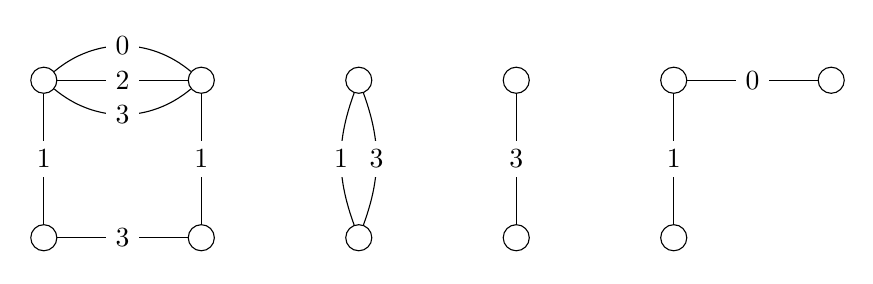
\begin{tikzpicture}

        \begin{scope}[every node/.style={circle,draw}]
          \node (1)  at (0,2)  {};
          \node (2)  at (0,0)  {};
          \node (3)  at (2,2)  {};
          \node (4)  at (2,0)  {};
          \node (5)  at (4,2)  {};
          \node (6)  at (4,0)  {};
          \node (7)  at (8,2)  {};
          \node (8)  at (8,0)  {};
          \node (9)  at (6,2)  {};
          \node (10) at (6,0)  {};
          \node (11) at (10,2) {};
        \end{scope}

        \begin{scope}[every node/.style={fill=white}]

          \begin{scope}[every edge/.style={draw}]
            \path (1)  edge[bend left=40] node {$0$} (3);
            \path (7)  edge node {$0$} (11);
            \path (1)  edge node {$1$} (2);
            \path (3)  edge node {$1$} (4);
            \path (5)  edge[bend right=20] node {$1$} (6);
            \path (7)  edge node {$1$} (8);
            \path (1)  edge node {$2$} (3);
            \path (1)  edge[bend right=40] node {$3$} (3);
            \path (2)  edge node {$3$} (4);
            \path (5)  edge[bend left=20] node {$3$} (6);
            \path (9)  edge node {$3$} (10);
          \end{scope}
        \end{scope}

      \end{tikzpicture}
      \caption{}
    \end{center}
  \end{figure}

  \paragraph{}
  Les trois dernières arêtes de $\rho_2$ doivent servir à relier les trois composantes connexes du graphe ci-dessus, sachant que l'arête 0 ne peut être relié à rien et qu'on ne sait créer que deux branches sur le carré alterné. Il y a donc 2 possibilités (une seule branche) plus 2 possibilités (deux branches, la branche avec $\rho_0$ ne contient aucune autre composante) plus 2 possibilités (deux branches, la branche avec $\rho_0$ contient deux composantes). On a donc exactement 6 possibilités.

\end{proof}
